\documentclass[11pt]{article}%
%%%%%%%%%%%%%%%%%%%%%%%%%%%%%%%%%%% Packages
\input ../../input/input-packages.tex

%%%%%%%%%%%%%%%%%%%%%%%%%%%%%%%%%%% Document data
\input ../../input/input-data.tex

\def\dochomework{}
\def\hw{GRE Notes} % Change document homework header
\def\docdate{2021/07/24} % Change document date
\def\docphone{+1.772.444.2710} % Change phone number

%%%%%%%%%%%%%%%%%%%%%%%%%%%%%% Macros
\input ../../input/input-macros.tex

%%%%%%%%%%%%%%%%%%%%%%%%%%%%%% Headers & footers
\input ../../input/input-header-footer.tex

%%%%%%%%%%%%%%%%%%%%%%%%%%%%%% Document style
\input ../../input/input-style.tex

%%%%%%%%%%%%%%%%%%%%%%%%%%%%%% Table of contents / index / bibliography
\input ../../input/input-toc-idx-bib.tex

%%%%%%%%%%%%%%%%%%%%%%%%%%%%%% Points and solutions
\input ../../input/exam-points-solutions.tex
%\printanswers% to print solutions

\begin{document}
\setlength{\baselineskip}{1.2\baselineskip}%
\setlength{\abovedisplayskip}{0pt}
\setlength{\abovedisplayshortskip}{0pt}
\begin{multicols*}{2}

%%%%%%%%%%%%%%%%%%%%%%%%%%%%%%%%%%%%%%%%%%%%%%%%%%%%%%%%%%%%%%%%%%%%%%
\prob{Proportionalities}
A relationship involving a \textit{product} (multiplication and division) equal to a \textit{constant}, the factors of that product must vary proportionately for the product to remain constant.

\begin{align*}
\multicolumn{4}{c}\text{\bf Directly Proportional} & \multicolumn{4}{c}\text{\bf Inversely Proportional} \\
\Aboxed{A &= kB} && k = \text{constant} & \Aboxed{C &= \frac{k}{D}} && k = \text{constant} \\
\frac{A}{B} &= k && \div B & CD &= k && \times D \\
\frac{\frac{2}{2} A}{\frac{2}{2} B} &= k && \frac{\frac{2}{2}}{\frac{2}{2}} = 1 & \frac{5}{4}C \frac{4}{5}D &= k && \frac{5}{4} \times \frac{4}{5} = 1 \\
\multicolumn{4}{c}\text{$A$ \& $B$ $\times$ same factors} & \multicolumn{4}{c}\text{$C$ \& $D$ $\times$ reciprocal factors} \\
\end{align*}
A memorable proportional relationship (from chemistry) is the \textit{Ideal Gas Law}: $\boxed{PV = nRT}$ where $R$ is the Ideal Gas Law \textit{constant}.
\begin{align*}
 &&\multirow{2}{*}{
 \begin{tabu}{l}
 P = \text{Pressure} \\
 V = \text{Volume} \\
 n = \text{Moles (\# of molecules)} \\
 T = \text{Temperature} \\
 R = \text{Ideal Gas Law} \textit{constant}
 \end{tabu}}\\
\Aboxed{PV &= nRT} & \\
\frac{PV}{nT} &= R \\
\end{align*}
So, for example...\begin{itemize}
\item If the \textbf{P}ressure increases, the \textbf{T}emperature must \textit{increase} (directly proportional) for everything else to remain constant. \item If the \textbf{V}olume increases, the \textbf{T}emperature must \textit{increase} (directly proportional) for everything else to remain constant. \item If the \textbf{P}ressure increases, the \textbf{V}olume must \textit{decrease} (inversely proportional) for everything else to remain constant. 
\item If the \textbf{V}olume increases, the \textbf{P}ressure must \textit{decrease} (inversely proportional) for everything else to remain constant. 
\item \etc
\end{itemize}

\divider

\prob{Pythagorean Theorem}
In a right triangle, with legs $a$ \& $b$ and hypotenuse (the longest side) $c$, $\boxed{a^{2} + b^{2} = c^{2}}$. \textit{Pythagorean triples} are right triangles with integer values for $a$, $b$, \& $c$. Memorize the most common ones below. Every odd number is the shortest leg of a Pythagorean triple where the longer sides are consecutive integers.

\begin{tabu} to \columnwidth{ccc|c}
 \multirow{6}{*}{\begin{tikzpicture}[align=center]%right triangle
 \coordinate (A) at (0,0);
 \coordinate (B) at (0,4);
 \coordinate (C) at (3,0);
 \draw (A) -- (B) node[above left,midway] { $a$ };
 \draw (A) -- (C) node[below,midway] { $b$ };
 \draw (B) -- (C) node[above right,midway] { $c$ };
 \tkzMarkRightAngle (B,A,C);
\end{tikzpicture}} 
 & \multicolumn{3}{c}{\textbf{Pythagorean Triples}} \\
 & $a$ & $b$ & $c$ \\\cline{2-4}
 & 3 & 4 & 5 \\
 & 5 & 12 & 13 \\
 & 7 & 24 & 25 \\
 & 8 & 15 & 17 \\
\\\\
\end{tabu}

\divider

\prob{Special Right Triangles}
\begin{tabu} to \columnwidth{cccc}
 \multirow{7}{*}{\begin{tikzpicture}[align=center]%half a square
 \coordinate (A) at (0,0);
 \coordinate (B) at (0,3);
 \coordinate (C) at (3,3);
 \coordinate (D) at (3,0);
 \draw [draw,decoration={markings, mark=at position 0.5 with {\node[transform shape] {$\vert$};}}]
 (A) edge[decorate] (B)
 (B) edge[decorate] (C)
 (C) edge[decorate] (D)
 (A) edge[decorate] (D);
 \draw (A) -- (C) node[above left,midway] { $\sqrt{2}$x };
 \draw (C) -- (D) node[right=0.125cm,midway] { $x$ };
 \draw (A) -- (D) node[below=0.125cm,midway] { $x$ };
 \draw[dashed] (A) -- (B);
 \draw[dashed] (B) -- (C);
 \tkzMarkRightAngle (A,B,C);
 \tkzMarkRightAngle (A,D,C);
\end{tikzpicture}} 
 & \multicolumn{2}{c}{\textbf{Half a Square}} \\
 & \multicolumn{2}{c}{Isosceles Right $\Delta$} \\
 & \multicolumn{2}{c}{$45^{\circ}$ - $45^{\circ}$ - $90^{\circ}$ $\Delta$} \\\cline{2-3}
 & $a^{2} + b^{2}$ &$= c^{2}$ \\ 
 & $\left(x\right)^{2} + \left(x\right)^{2}$ &$= \left(\sqrt{2}x\right)^{2}$ \\
 & $x^{2} + x^{2}$ &$= \left(\sqrt{2}\right)^{2}x^{2}$ \\
 & $2x^{2}$ &$= 2x^{2}$ \\
\end{tabu}

Remember: $\boxed{x,\;x,\;\sqrt{2}x}$
\begin{itemize}\item $\sqrt{2}x$ is the hypotenuse, since it is the longest side ($\sqrt{2} > 1$) \item $x$ \& $x$ are the legs, since half a square is an \textit{isosceles right triangle}.
\end{itemize}
\bigskip

\begin{tabu} to \columnwidth{cccc}
 \multirow{7}{*}{\begin{tikzpicture}[align=center]%half an equilateral triangle
 \coordinate (A) at (1.5,0);
 \coordinate (B) at (1.5,2.6);
 \coordinate (C) at (3,0);
 \coordinate (D) at (0,0);
 \draw [draw,decoration={markings, mark=at position 0.5 with {\node[transform shape] {$\vert$};}}]
 (A) edge[decorate] (D)
 (A) edge[decorate] (C);
 \draw [draw,decoration={markings, mark=at position 0.5 with {\node[transform shape] {$\parallel$};}}]
 (B) edge[decorate] (D)
 (B) edge[decorate] (C);
 \draw (A) -- (B) node[left,midway] { \\\\$\sqrt{3}$y };
 \draw[dashed] (B) -- (D) node[above left,midway] { $2y$ };
 \draw (B) -- (C) node[above right,midway] { $2y$ };
 \draw (A) -- (C) node[below=0.125cm,midway] { $y$ };
 \draw[dashed] (D) -- (A) node[below=0.125cm,midway] { $y$ };
 \tkzMarkRightAngle (C,A,B);
\end{tikzpicture}} 
 & \multicolumn{2}{c}{\textbf{ Half an Equilateral} $\Delta$} \\
 & \multicolumn{2}{c}{$30^{\circ}$ - $60^{\circ}$ - $90^{\circ}$ $\Delta$} \\\cline{2-3}
 & $a^{2} + b^{2}$ &$= c^{2}$ \\ 
 & $\left(y\right)^{2} + \left(\sqrt{3}y\right)^{2}$ & $= \left(2y\right)^{2}$ \\
 & $y^{2} + \left(\sqrt{3}\right)^{2}y^{2}$ &$= 2^{2}y^{2}$ \\
 & $y^{2} + 3y^{2}$ &$= 4y^{2}$ \\
 & $4y^{2}$ &$= 4y^{2}$ \\
\end{tabu}

Remember: $\boxed{x,\;\sqrt{3}x,\;2x}$
\begin{itemize}\item $2x$ is the hypotenuse, since it is the longest side ($2 > \sqrt{3} > 1$) \item $x$ \& $\sqrt{3}x$ are the legs, since they are the other two.
\end{itemize}

\divider%\vfill\null\columnbreak

\prob{Fencepost Problems}
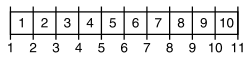
\includegraphics{./250px-Fencepost_error.svg.png}
From \href{https://en.wikipedia.org/wiki/Off-by-one_error\#Fencepost_error}{Wikipedia}, `If you build a straight fence 30 meters long with posts spaced 3 meters apart, how many posts do you need? The common answer of 10 posts is wrong. This response comes from dividing the length of the fence by the spacing apart from each post, with the quotient being erroneously classified as the number of posts. In actuality, the fence has 10 sections but 11 posts. In this scenario, a fence with $n$ sections will have $n + 1$ posts. Conversely, if the fence contains $n$ posts, it will contain $n - 1$ sections.'

The rule of thumb is: to find the number of numbers between $M$ and $N$, you must use $N - M + 1$. So, how many numbers are there between 47 and 54? $54 - 47 + 1 = 8$. Counting: 47, 48, 49, 50, 51, 52, 53, 54 is eight.

\divider

\prob{Standard Deviation}
The \textit{standard deviation} of a set of data is a measure of the average distance of data values from the mean value of the data. The formula for the standard deviation $\sigma$ of $N$ data values $X_{i}$ whose mean is $\overline{X}$ is:
\begin{align*}
\sigma = \sqrt{\frac{\sum_{1}^{N}\left(X_{i} - \overline{X}\right)^{2}}{N}}
\end{align*}

From \href{https://www.desmos.com/calculator/dyjchcbu3s}{Desmos}, a GRE problem asked whether changing certain data values changes the standard deviation? In this case, the values above and below the mean --- and their distances greater than and less than the mean --- are the same, so the standard deviations are equal (without calculation!).

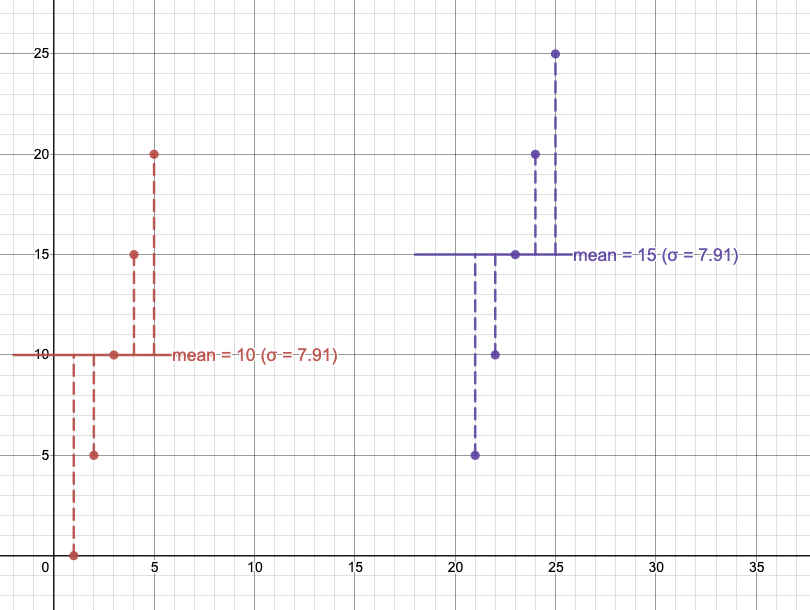
\includegraphics[width=\columnwidth]{./desmos-std-dev.png}

From the \href{https://circuitcellar.com/research-design-hub/basics-of-design/making-heads-or-tails-of-rms-measurements/}{Circuit Cellar}, the classic normal distribution percentage graph says $\pm 1\;\sigma$ is $\boxed{\pm 34.1\%}$ from the mean, $\pm 2\;\sigma$ is $34.1\% + \boxed{13.6\%} = \pm 47.7\%$ from the mean, and $\pm 3\;\sigma$ is $47.7\% + \boxed{2.1\%} = \pm 49.8\%$ from the mean.
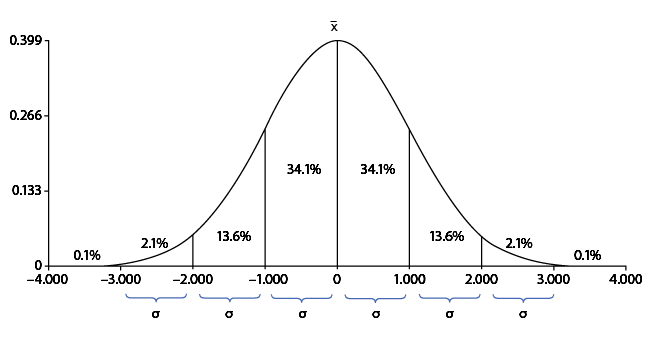
\includegraphics[width=\columnwidth]{./cc-std-dev-percent.png}

Also from the \href{https://circuitcellar.com/research-design-hub/basics-of-design/making-heads-or-tails-of-rms-measurements/}{Circuit Cellar}: `If you take any Gaussian-shaped histogram, and cut it halfway from the maximum, you will get a width of 2.355 times the standard deviation. This value is called the \textit{full width at half maximum} (FWHM).'
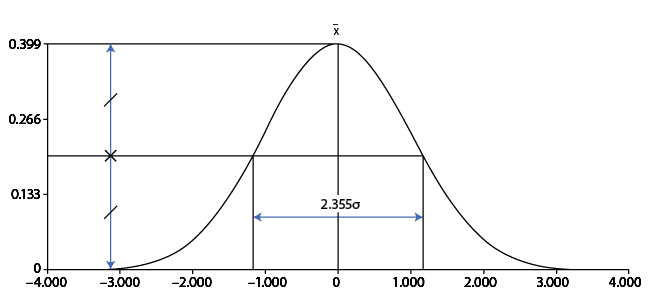
\includegraphics[width=\columnwidth]{./cc-fwhm.png}

\divider

\prob{Circular Arc Lengths}
The ratio of the central angle ($\theta$) to the entire circle ($360^{\circ}$) is proportional to the ratio of the arc length ($s$) to the entire circumference ($C$).

\newcommand\TR{3}
\begin{center}\begin{tikzpicture}[align=center]%circular arc
 \coordinate (C) at (\TR,\TR);
 \coordinate (A) at (\TR+\TR,\TR);
 \coordinate (B) at (0.866*\TR+\TR,0.5*\TR+\TR);
 \draw (C) circle (0.02*\TR);
 \draw (C) circle (\TR);
 \draw (C) node[left] { $C$ } -- (A) node[below,midway] { $r$ } node[right] { $A$ };
 \draw (C) -- (B) node[above right] {$B$};
 \draw[red] (\TR+\TR,\TR) arc (0:30:\TR) node[black,right,midway] { $s$ };
 \draw[-latex] (0.5*\TR + \TR,\TR) arc (0:30:0.5*\TR) node[right,midway] { $\theta^{\circ}$ };
 \draw[-latex,style=dashed] (0.25*\TR + \TR,\TR) arc (0:360:0.25*\TR) node[left,midway] { $360^{\circ}$ };
\end{tikzpicture}\end{center}
\begin{align*}
C = \pi D = 2 \pi r \\
\boxed{\frac{\theta^{\circ}}{360^{\circ}} = \frac{s}{C}}
\end{align*}

\divider

\prob{Linear Equations}
Linear relationships involve \textit{slope}. The slope is a constant that determines the amount of change in $y$ for a given change in $x$. The slope is always $\boxed{m = \frac{\text{rise}}{\text{run}}}$.

\begin{description}
\item[Slope-Intercept] $\boxed{y = mx + b}$ \\ Use when you know the slope $m$ and the $y$-intercept $\left( 0, b \right)$.
\item[Point-Slope] $\boxed{\left( y - y_{1} \right) = m \left( x - x_{1} \right)}$ \\ Use when you know the slope $m$ and any point $\left( x_{1}, y_{1} \right)$.
\item[Standard] $\boxed{Ax + By = C}$ \\ Use when the equation is written in standard form. In that case, $\boxed{m = \frac{-A}{B}}$ (and the $y$ value of the $y$-intercept $\left( 0, b \right)$ is $b = \frac{C}{B}$ and the $x$ value of the $x$-intercept $\left( a, 0 \right)$ is $a = \frac{C}{A}$).
\end{description}

\divider

\prob{`Cross Multiplication' versus `Canceling'}
\begin{tabu} to \linewidth {X[c]X[c]}
\textbf{Cross Multiply} only across an $=$ sign & \textbf{Cancel} only in a quotient \\\hline
$\frac{3}{11} = \frac{x}{33}$ & $\frac{3}{11} \times \frac{x}{33}$ \\
$\frac{3}{1} \mathrlap{\searrow}\mathrlap{\swarrow}= \frac{x}{3}$  & $\frac{\cancelto{1}{3}}{11} \times \frac{x}{\cancelto{11}{33}}$ \\
$1 \times x = 3 \times 3$ & $\frac{1}{11} \times \frac{x}{11}$ \\
$x = 9$ & $\frac{x}{121}$ \\
\end{tabu}
For \text{any} equation, always `do the same thing to both sides.'

\divider

\prob{Powers of Small Integers}
Memorize these.
\begin{align*}
2^{0} &= 1 & 3^{0} &= 1 & 4^{0} &= 1 & 5^{0} &= 1 & 6^{0} &= 1 \\
2^{1} &= 2 & 3^{1} &= 3 & 4^{1} &= 4 & 5^{1} &= 5 & 6^{1} &= 6 \\
2^{2} &= 4 & 3^{2} &= 9 & 4^{2} &= 16 & 5^{2} &= 25 & 6^{2} &= 36 \\
2^{3} &= 8 & 3^{3} &= 27 & 4^{3} &= 64 & 5^{3} &= 125 & 6^{3} &= 216 \\
2^{4} &= 16 & 3^{4} &= 81 & 4^{4} &= 256 & 5^{4} &= 625 \\
2^{5} &= 32
\end{align*}
Why is $256$ my favorite number?
\begin{align*}
2^{8} = 4^{4} = 16^{2} = 256^{1} = \left(\left(\left( 2 \right)^{2}\right)^{2}\right)^{2}
\end{align*}
...and every one of those numbers is power of 2!

\divider

\prob{Rules of Exponents}
\textit{Rules of products of exponents with like bases \textbf{only}}. In $b^{e}$, $b$ is the base and $e$ is the exponent.
\begin{align*}
x^{a} \times x^{b} &= x^{a + b} && \text{product is sum of exponents} \\
x^{a} \div x^{b} &= x^{a - b} && \text{quotient is difference of exponents} \\
\left( x^{a}\right)^{b} &= x^{a \times b} && \text{power-of-power is product of exponents} \\
x^{-1} &= \frac{1}{x} && \text{negative exponent is reciprocal}
\end{align*}

For example:
\begin{align*}
y^{2} \times y^{3} = \left( y \times y \right) \times \left( y \times y \times y \right) &= y^{6} = y^{2 + 3} \\
\frac{y^{2}}{y^{3}} = \frac{\left( y \times y \right)}{\left( y \times y \times y \right)} = \frac{\bcancel{y} \times \bcancel{y}}{\bcancel{y} \times \bcancel{y} \times y} = \frac{1}{y} &= y^{-1} = y^{2 - 3} \\
\left( y^{2} \right)^{3} = \left( y \times y \right) \times \left( y \times y \right) \times \left( y \times y \right) &= y^{6} = y^{2 \times 3}
\end{align*}
These rules work even if the exponents are not integers. (However, fractional exponents are radicals.)

\divider

\prob{Rules of Radicals}
\hwnote{More \href{https://en.wikipedia.org/wiki/To_come_(publishing)}{TK}}

\divider

\prob{Permutations}

Combinatorics is described in detail in a paper I wrote for graduate school. Download it here: \url{https://dcpetty.github.io/latex/math/20100630-uml-04.535-final-project.doc}.

\divider

\end{multicols*}
\end{document}
